\section{Grounding referring expressions}
\label{sec:preexperiments}

This chapter serves two purposes.
First, the generated dataset from the precious section is validated.
For this, models are trained to both generate referring expressions of the target object and understand existing referring expressions.
A success of these experiments indicates that the target objects in the datasets are possible to refer to and the datasets can be used in more complex setups in language games.

Secondly, the experiments in this chapter provide the basis for the setup of the agents in the language games.
Language games are very complex setups for machine learning models.
The models need to solve multiple tasks at the same time in order to solve the overall problem.
For instance, in a simple setup of a game two agents are involved.
The first agent, the sender, is shown a scene with objects and needs to communicate one target object to the other agent, the receiver.
The receiver is shown the same scene and needs to identify the target object with respect to the message of the sender.
In this case, the sender first needs to learn to encode the scene, all objects and their attributes, as well as the information about the target object into its own game specific space.
In a next step it needs to learn how to translate this encoding into a message that is sent to the receiver.
The receiver then needs to learn to decode this message, after which it needs to learn how to combine the decoded message with its own encoding of the scene and objects.
And finally it needs to learn how to identify the target object with this information.
There are many points of possible failure to train the agents.
% SD: This should go at the beginning where language games with neural agents are introduced.
% DK: TODO

For this reason, we decided to divide the main problem and let the models learn simpler subtasks and increase the complexity step by step.\footnote{\href{https://github.com/DominikKuenkele/MLT\_Master-Thesis}{https://github.com/DominikKuenkele/MLT\_Master-Thesis}}
This will give a very detailed overview where the models struggle to learn and in which ways they can be improved.
Mainly, the tasks are separated into language games with two agents and classical machine learning tasks without any communication, namely only one 'agent' that solves the task alone.
With this division, we can analyze the learning of the encodings of the scenes separately from the learning of producing and decoding messages.

% TODO maybe move to front...
The final objective of this thesis is to find out, how agents can communicate about relations of objects based on their attributes, namely how to generate and understand referring expressions.
Because of that, the first experiments focus on extracting information from images and combining them with structured knowledge about the objects.
Here, we structured the experiments into three levels.
In the first level, the models are trained to learn the position of objects in the image and attend to specific regions of the image, by understanding a referring expression of the target object.
% SD: This is a natural language understanding or reference resolution task.
% DK: TODO maybe put into methods...
In the second level, the models are trained to differentiate objects in the scene from each other, again by understanding referring expressions.
% SD: Object identification task
% DK: TODO
In the last level, the models are trained to generate referring expressions, more specifically the models learn to caption and describe objects in the image.
% SD: Referring expression generation task
% DK: TODO
These combined experiments should lay the basis for how to build up the agents in the language games.
% SD: We are validating the dataset on 3 tasks
% DK: TODO

\subsection{Object identification}
\label{sec:object-identification}
\subsubsection*{Setup}

In a first task a neural model is trained to discriminate multiple objects from each other.
Hereby, the model is shown bounding boxes of all objects in the scene as well as a description of the target object.
The model needs to combine all information and then point to the correct bounding box.
This task forces the model to extract visual features from the objects in the shown inputs and connect them to a representation of human given attributes.
Since the model is shown only bounding boxes around each object rather than the whole scene, geometric information about the objects' locations doesn't play a role for the success in this task.

In a first step, bounding boxes are extracted from each scene.
Each bounding box is a square with a side length of 96 pixels around the center coordinates of each object.
By doing this large objects in the front of the scene fill the bounding box completely, while smaller objects in the back of the scene contain some space around them.
They also might contain noise in the form of parts of adjacent objects.
Preliminary experiments indicated however that a more complex method for extracting the bounding boxes, depending on spatial position in the scene to reduce the noise didn't improve the results.
Therefore, bounding boxes in this thesis rely on the former simpler approach.
Since, each bounding box will be passed through on of the feature extractors, described in section \ref{sec:feature-extractors} they need to be normalized first.
As described in \citep{He2016,Simonyan2015}, the bounding boxes are resized to 256 pixels for the shorter side, then cropped around the center to a square of 224 \times\ 224 pixels.
Finally, the RGB channels are normalized, by subtracting the means (0,485; 0,456; 0,406) and dividing the result by the standard deviation (0,229; 0,224; 0,225) for each channel respectively.
The array of bounding boxes is padded with matrix of zeros to the maximum possible number of objects present in a scene across the dataset.
For the 'Dale-2' dataset, this corresponds to a maximum of two bounding boxes, 5 bounding boxes for the 'Dale-5' dataset and 10 for the 'CLEVR color' dataset.
For each sample in the dataset the bounding boxes are shuffled.

The attributes of the target object are encoded as one-hot encodings.
There is a three-dimensional vector encoding the \emph{shape}, an eight-dimensional vector encoding the \emph{color} and a two-dimensional vector encoding the two different \emph{sizes}.
The values of each dimension of these vectors can either be zero or one, depending on the attributes of the target object.
These three encodings of the attributes are then concatenated to a vector with 13 dimensions.

\begin{figure}[ht]
    \centering
    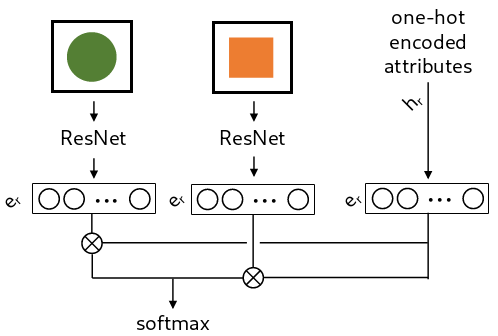
\includegraphics[width=.5\linewidth]{figures/arch_bounding_box_classifier.png}
    \caption{Simplified architecture of the object identification task}
    \label{fig:bounding_box_classifier_architecture}
    % SD: I haven't commented on this before, but let us be very careful in naming all meta-paramaters of the models in the text or in caption: how many layers, how many dimensions, etc. The reader should be able to replicate the code and the experiment from this. You can do this in the caption which is a longer explanation or in the text itself.
    % DK: TODO
\end{figure}

The model, the \emph{object identifier} is split into two parts.
First, each normalized bounding box of the sample is passed through \emph{ResNet-avg}.
The preceding layers \emph{ResNet-1} to \emph{ResNet-4} couldn't be compared due to memory restrictions on the GPU.
A deeper analysis of the effects of different feature extractors will be done in the following chapters.
The resulting vector is flattened and projected to the embedding dimension $e$ via a linear layer.
% SD: This is quite low? Why only 10?
% DK: different embedding sizes are tested (done)
Correspondingly, the one-hot vector of the attributes is projected to the same embedding dimension with another linear layer.
In the second part, each bounding box is combined with the representation of the attributes.
By bringing both vectors to the same embedding size, the dot product between each embedded bounding box and the embedded attributes can be calculated.
A high correlation between the attributes and the object should result in a high dot product, while a low correlation results in a lower dot product.
The model can so learn to connect the object representation with the attributes.
The dot products are concatenated and form a vector with as many dimensions as objects present.
The \emph{softmax} function is applied over the resulting vector, which returns a probability distribution over all objects; the model points to the object with the highest probability.
% The model then points to an object, using the \emph{softmax} function over this resulting vector.

The experiments are conducted with the following hyperparameters: a learning rate of $2\times10^{-4}$, a batch size of 32 samples and 30 epochs, \emph{Adam} \citep{Kingma2015} as optimizer.
The number of epochs was chosen manually after identifying when the loss as well as the test accuracies didn't improve significantly.
8000 randomly selected samples are used for training, the remaining 2000 samples for testing.
The loss is calculated using cross entropy.
The following embedding dimension $e$ are compared: 2, 10, 50, 100, 500, 1000.
% SD: So, the output of this model is a vector of 0 and 1s, with the 1 identifying the corrct object (or the other way around?).
% DK: the output is a probability distriution over all objects (inserted above; done)

The object identification task is trained on all datasets that include more than one object in each sample, namely the 'CLEVR color', 'Dale-2' and 'Dale-5' dataset.
Random baselines for each dataset would yield accuracies of 10\%, 50\% and 20\% respectively.
% excluding the 'CLEVR single'.
% SD: Why not?
% DK: because there is only one object in the input, and therefore only one possible guess. The model can't point to a distractor (adressed; done)
The 'Dale' datasets are directly comparable to each other for the similar setup of their creation.
Especially interesting is the effect of the increasing the number of distractors and the growing number of attributes that are needed to discriminate the objects.

\subsubsection*{Results}
Table \ref{tab:results:bounding_box_classifier} lists the accuracies of the models' predictions after 30 epochs for all three different datasets and different embedding sizes $e$.

\begin{table}[ht]
    \centering
    \begin{tabular}{c|c|c|c}
        \toprule
               & \textbf{Dale-2}   & \textbf{Dale-5}   & \textbf{CLEVR Color} \\\cmidrule(lr){2-2}\cmidrule(lr){3-3}\cmidrule(lr){4-4}
        $e$    & \textbf{Accuracy} & \textbf{Accuracy} & \textbf{Accuracy}    \\\midrule
        {2}    & {92\%}            & {72\%}            & {40\%}               \\
        {10}   & \textbf{100\%}    & {94\%}            & {92\%}               \\
        {50}   & {99\%}            & \textbf{95\%}     & \textbf{94\%}        \\
        {100}  & \textbf{100\%}    & \textbf{95\%}     & {93\%}               \\
        {500}  & \textbf{100\%}    & \textbf{95\%}     & {93\%}               \\
        {1000} & \textbf{100\%}    & {94\%}            & \textbf{94\%}        \\
        \bottomrule
    \end{tabular}
    \caption{Accuracy scores of the object identifier after 30 epochs: $e$ are different embedding sizes}
    \label{tab:results:bounding_box_classifier}
\end{table}

The first trend that is visible is that fewer distractor increase the accuracy of the model.
The model achieves almost perfect accuracy in all configurations for the \emph{Dale 2} dataset with only two objects.
With five objects in the \emph{Dale-5} dataset, the accuracy drops to 95\% and with a maximum possible number of 10 objects in the \emph{CLEVR color} dataset the model only achieves 94\% in the best configuration.
This is not very surprising, since the model has a higher chance of predicting a wrong object, given the random baselines of 50\%, 20\% and 10\%.
Furthermore, when more objects are shown to the model, more attributes are needed to discriminate the target object from the distractor, since it is more likely that the distractors share attributes with the target object.
The task is getting therefore more challenging.

A second conclusion is that the model needs a certain embedding space, to represent the features of each image.
Across all dataset, an embedding space of only 2 dimensions result in a much lower performance compared to the best configuration.
Even though the model is still able to achieve an accuracy of 30\% to 50\% points over the random baseline, this shows that a bigger embedding size is beneficial to extract and represent the features of the objects.
Between 50 and 1000 dimensions, the model performs the best and varies only by 1\% point, which may be due to different random initialization of the weights in the model.

In conclusion, the model is able to learn to discriminate the objects based on the visual appearance.
The model can generate these high results, even with its relatively simple architecture.
In this architecture, the model doesn't compare the objects directly to each other, but each object is only associated with the attribute encodings.
A more complex architecture, in which the model is additionally tasked to discriminate the objects directly from each other might even improve the results.
% SD: The model is able to leatn to discriminate objects based on visual appearance.
% DK: (done)

\subsection{Referring expression generation}
\label{sec:referring_expression_generation}
\subsubsection*{Setup}

Opposed to the previous experiment, where the focus lied on extracting visual features, the model is now tasked to generate referring expressions.
This is done in two setups.
The first setup uses bounding boxes as in the previous section as input, where the model needs to describe the target object of one of the bounding boxes.
In the second setup, the model is presented with the complete image and therefore also needs to accommodate to geometric information of the scene.

The bounding boxes are extracted and normalized in the same way as for the object identification task.
Since for the second setup, the images will also be passed through the feature extractors, they are normalized as well in like manner.
The referring expressions for the target object are generated using the incremental GRE-algorithm, described in section \ref{GRE}.
By this, the model needs to describe the target object with respect to the distractor objects.
There are some minor additions concerning the padding of the referring expression.
As before, the referring expression is padded to a number of three tokens, corresponding to the maximum of three attributes.
However, there are three different ways how the padding is applied.
First, the referring expression are, as usual in captioning tasks padded at the end with a specified padding token.
A problem could arise when the referring expression is not viewed as a natural language sentence, but as slots filled with tokens.
More specifically, following the GRE-algorithm, the last token in the referring expression is always the shape.
The second last token if existing describes the color, while the third last token if existing describes the size.
As soon as this sequence is padded at the end, these slots disappear.
A referring expression that only describes the shape, such as \emph{cube} will be padded to \emph{cube <pad> <pad>}, where the third last slot is filled up with the shape instead of the size.
Since this task is not focussing on producing natural language with a correct grammar, but focuses instead on extracting attributes, having a slot structure could help the model to express the extracted attributes correctly.
For this reason, the second method of padding the referring expression is prepending the referring expression with padding tokens.
By this, the positions of the slots are preserved and if not specified just filled with a padding token.
Each slot has always the same semantic value, e.g. the last slot always contains the shape of an object.
This can be done since the referring expressions are not free text, but instead the structure and the possible content is given by the dataset.
This method might help the model to learn the correct referring expressions.
% SD: Slots have the same semantic value, i.e. the last slot is the object type. We can do this because we know the structure of the descriptions in this dataset and because we hope this will help the learning. Also, we are thinking of generation based on slots.
% DK: (addressed; done)
The last variation concerns the order of producing each token.
When the referring expressions are prepended, the model would need first produce two padding tokens, before it finally can produce a much more meaningful token for the shape.
This could be difficult to learn for a model, as the longer a sequence of tokens is, the more information about the beginning of the sequence gets lost.
Even though a sequence of just three tokens may not be long enough for this factor to be a problem, we experimented to reverse the referring expression.
% SD: We... I sounds more like you are writing a lab report with casual language but here you want to be more formal.
% DK: (done)
Instead of producing for instance \emph{<pad> green sphere} as correct in English, the model would now need to produce \emph{sphere green <pad>}.
Notice that the padding token is again at the end of the generation, but the order of slots as well as the amount of information in the referring expression are still preserved.

This task inherently involves learning human knowledge and natural language structure.
Nonetheless, this helps to understand more detailed if and how the model discriminates objects.
Can the model solve the task, or do specific attributes used by humans pose challenges to the model?
% Does it rely on the same attributes humans are using, or does it find other important differences, or is it not able to solve the task at all?
% SD: In this case it should be using the same attributes as humans as we are training it on human labels.
% DK: (rephrased; done)

% TODO include figure

In the first setup, the \emph{bounding box RE generator}, the model receives the bounding boxes as input.
The first bounding box is always the target object, while the remaining bounding boxes are shuffled.
As in the previous experiment, each bounding box is passed through \emph{ResNet-avg} and projected afterwards to an image embedding dimension $e$ with a linear layer.
All thus encoded bounding boxes are concatenated and again compressed to the decoder output dimension $LSTM_o$ using another linear layer.
This representation of all objects serves as the initial hidden state of an LSTM, which generates the referring expression.
Tokens used in the LSTM are embedded with embedding dimension $LSTM_e$.
During training, teacher forcing is applied by using embeddings of the ground truth tokens as the input sequence for the LSTM, instead of the output of the LSTM.
The output of the LSTM is passed through a linear layer at each step to determine logits over the symbols of the vocabulary.
During testing, the LSTM is always forced to generate three tokens, with an embedded start-of-sequence token as first input to the LSTM.
Each token in the sequence is determined greedily, by selecting the highest logit in the output of each step in the LSTM.

\begin{figure}[ht]
    \centering
    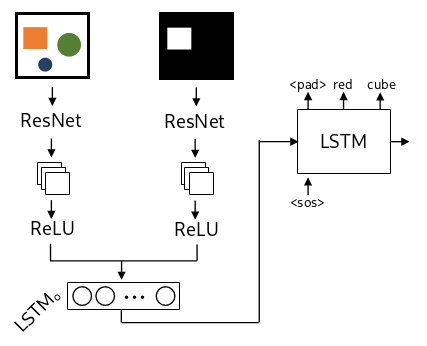
\includegraphics[width=.5\linewidth]{figures/arch_caption_generator.png}
    \caption{Simplified architecture of the masked caption generator}
    \label{fig:caption_generator_architecture}
\end{figure}

In the second setup two different models are compared against each other.
The first model, the \emph{basic RE generator} acts as the baseline and only receives the complete image as the input.
The image is passed through \emph{ResNet-3} and subsequently processed by additional convolution layers, described in section \ref{sec:image-processing}.
The resulting vector is then reduced to decoder output dimension $LSTM_o$ by a linear layer and as for the bounding boxes acts as the initial hidden state for the LSTM.
The LSTM is trained in the same way as above.

Using this approach, the model doesn't have any information about the target object and is therefore expected to produce referring expressions for a randomly selected object on the scene.
Therefore, it is extended in a second step with attention to the target object, the \emph{masked RE generator}.
% SD: You add attention to the target object.
% DK: (added; done)
A masked version of the image is created and passed to the model.
For this, a fixed size squared area of 96 \times\ 96 pixels around the center of the target object is filled in white, while the rest of the image is filled in black.
Both original and masked image are processed together with convolutional layers as described in section \ref{sec:image-processing}.
% SD: This is normally implemented as a filter of 1 and 0 corresponding to pixels. As such it then corresponds to attention, cf. paper with Mehdi.
% DK: (QUESTION)
The result is then again projected to the decoder output dimension $d$ by a linear layer and then used as the initial hidden state for the LSTM.
This should point the model towards which object to describe and discriminate from the distractors.

For both setups, the same hyperparameters as in the previous experiments are used: a learning rate of $2\times10^{-4}$, a batch size of 32 samples and 30 epochs, \emph{Adam} \citep{Kingma2015} as optimizer.
8000 randomly selected samples are used for training, the remaining 2000 samples for testing.
The loss is calculated using cross entropy.
Table \ref{tab:variables-reference-expression-generation} shows which variables are compared for each model:

\begin{table}[ht]
    \centering
    \begin{tabular}{lccc}
        \toprule
                                  & $e$                & $LSTM_o$           & $LSTM_e$       \\
                                  & $[100, 500, 1000]$ & $[100, 500, 1000]$ & $[10, 15, 30]$ \\\midrule
        bounding box RE generator & \times             & \times             & \times         \\
        basic RE generator        & -                  & \times             & \times         \\
        masked RE generator       & -                  & \times             & \times         \\
        \bottomrule
    \end{tabular}
    \caption{Variables for each model where $e$ is the embedding dimension, $LSTM_e$ the embedding dimensions for tokens in the LSTM and $LSTM_o$ the output dimension of the LSTM}
    \label{tab:variables-reference-expression-generation}
\end{table}

As already discussed before, this task can be interpreted as a classification task rather than a natural language generation task.
The main reason for this is that the model is tasked to assign specific attributes to the target object instead of producing free text with a large vocabulary.
Following, we are interested in the classification mistakes the model makes.
For this, the model's success is validated on accuracy, recall and precision scores.
These are calculated in the following ways.
The first measure is the \textbf{overall accuracy} if the model predicted every word in the caption correctly.
% SD: This is too strict. if this is a generation task then we can use generation metrics. Those compare if the generated string as a whole is kind of similar to the target string, see ROUGE, METEOR, BERTscore.
% If this is a classification task, and it is, given that we know what type of word we expect in each slot, we could calculate accuracy per class, precision, recall, F-score. We could also calculate mean ranks for predicting words per classes, or acucracy at k- if the target word is in the k-top predictions.
% We could also take it a multi-class classification problem and how to calculate accuracy in this case, would need to check.
% DK: I agree that classification metrics refelct success better here (therefore I also used accuracy). These metrics would give a better overview, but I don't think there is time to implement it (QUESTION)
This gives a hint, how the model fares in general and if it is able to predict any of the attributes.
However, a 'false' prediction doesn't give much insight into why the model predicted a wrong caption.

It could be the case that the model predicted the correct shape, but wrong color.
Even worse, the model could have predicted more attributes than necessary to uniquely identify the target object and didn't follow the rules of the GRE-algorithm.
For instance, consider the scene in Figure \ref{fig:clevr-dale-5}.
% SD: Too far away, might be worth repeating here, you say still stay Fiigure 2d, repeated asFigure 6 here
% DK: TODO
The correct caption is \emph{cylinder}.
If the model would predict \emph{purple cylinder}, the accuracy determines it as false as captioning \emph{large purple cylinder} as well \emph{small green cube}.
The first two descriptions identify the target object perfectly, but the model only didn't learn to exclude unnecessary attributes.
To mitigate this, the accuracies for each class are included, as well as the macro average.
% SD: Is this figure for a particular class, i.e. object type, or do you then do something to individual accuracy, i.e. average them?
% DK: the metric is averaged over all samples (not by class). Might be definitly worth to do it class by class. Time? (QUESTION)
This can give a better understanding of the errors the model makes.
The same is done for \textbf{precision} and \textbf{recall}.

% SD: Very good If I understand this right this would be a case where the generated description describes another object better than the target and a human would identify that. So it is like false negatives in describing. Perhaps use another term for this: referring to a distractor? (since you are not measuring hwo individually the description fitts a distractor but only if the entire description could perfectly fit a distractor)
% DK: exactly. I added false negatives. But I would like to keep accuracy in the name, since that is what it is. maybe better distractor accuracy? (QUESTION)
With the \textbf{non-target accuracy}, we identify if the model described another object, which is not the target image.
This is basically an inverted accuracy score; the lower the score, the better the model fares.
By this it measures the false negative generated captions.
For this we generated captions for all the non-target objects and distractors in the images using the GRE-algorithm.
If the generated description of the model describes an object that is not the target object, it gets assigned 100\%.
If not, independently of describing the target object, no object, or one of the objects insufficiently, it gets assigned 0\%.
Using this measure, we can get an overview if the model's problem lies in extracting and relating attributes or in understanding which of the presented objects is the target object.

The caption generator models are trained on both 'Dale' datasets.
Again, each of these datasets increases the complexity of the description.
While the referring expression for the 'Dale-2' datasets are generally shorter, expressions of the 'Dale-5' datasets need to be more specific and use more attributes.
Furthermore, the model needs to attend to many more locations in the image at the same time to find discriminating factors between those.

\subsubsection*{Results}
Table \ref{tab:results:bb-re-generator} shows the \emph{overall accuracy}, \emph{F1 scores} for each word and the \emph{non-target accuracies} of the \textbf{bounding box RE generator} when trained on the \emph{Dale-2}, \emph{Dale-5} and \emph{CLEVR color} datasets.
As can be seen, the overall accuracies, in other words perfect matches of the generated referring expression depend very much on the dataset.
With the \emph{Dale-2} dataset, the model can achieve perfect matches in 99\% of the cases in its best configuration.
Also the \emph{CLEVR color} dataset allows the model to predict the correct referring expression in 93\% of the samples.
Opposed to that the model can only generate perfect referring expressions in 69\% of the samples of the \emph{Dale-5} dataset.
Looking at the \emph{non-target accuracy}, one of the problems can be identified for the \emph{CLEVR color} dataset.
Summing the \emph{non-target accuracy} and the \emph{overall accuracy}, one gets the accuracy that any of the shown object was described independently if it was the target object.
For the \emph{CLEVR color} dataset, this score lies at 96\% to 97\% in the best configurations, which means that the model described a shown object for almost all the samples.
In 3\% to 4\% of the cases, the model only picked the wrong object to describe.
This looks different for the \emph{Dale-5} dataset.
Here, the model describes only in 71\% of the cases one of the shown objects, 69\% the target object and 2\% a distractor.
The model therefore struggles more with the correct generation of words than with choosing, which object to describe.

When looking at the different configurations, in especially different values for $e$, $LSTM_o$ and $LSTM_e$, it can be seen that the results are not very different for the \emph{Dale-2} and \emph{CLEVR color} datasets.
However, bigger effects can be identified for the \emph{Dale-5} dataset.
Here, a low output dimension of the LSTM $LSTM_o$ tends to give lower scores.
This especially enhanced, when also the embedding dimensions of the tokens $LSTM_e$ is low.
Again, the image embedding size $e$ doesn't seem to have a big effect, when over 50 dimensions.
Indeed, the model achieves an accuracy of 69\% with all three tested embedding sizes.

\begin{table}[ht]
    \centering
    \begin{tabular}{ccc|ccc|ccc|ccc}
        \toprule
               &          &          & \multicolumn{3}{c}{\textbf{Dale-2}} & \multicolumn{3}{c}{\textbf{Dale-5}} & \multicolumn{3}{c}{\textbf{CLEVR color}}                                                                                               \\\cmidrule(lr){4-6}\cmidrule(lr){7-9}\cmidrule(lr){10-12}
        $e$    & $LSTM_o$ & $LSTM_e$ & \textbf{Acc.}                       & \textbf{F1}                         & \textbf{NT}                              & \textbf{Acc.} & \textbf{F1}    & \textbf{NT} & \textbf{Acc.} & \textbf{F1}    & \textbf{NT} \\\midrule
        {100}  & {100}    & {10}     & {97}                                & {97,67}                             & {1}                                      & {65}          & {88,17}        & {2}         & {92}          & {94,95}        & {3}         \\
        {100}  & {100}    & {15}     & {97}                                & {97,77}                             & {0}                                      & {62}          & {86,51}        & {2}         & {92}          & {94,45}        & {4}         \\
        {100}  & {100}    & {30}     & {98}                                & {97,81}                             & {1}                                      & {65}          & {87,97}        & {2}         & {92}          & {94,47}        & {4}         \\
        {100}  & {500}    & {10}     & {98}                                & {98,16}                             & {0}                                      & {67}          & {88,13}        & {2}         & {93}          & {95,18}        & {4}         \\
        {100}  & {500}    & {30}     & \textbf{99}                         & \textbf{98,57}                      & \textbf{0}                               & \textbf{69}   & \textbf{89,53} & \textbf{2}  & \textbf{93}   & \textbf{95,17} & \textbf{3}  \\
        {100}  & {1000}   & {10}     & {98}                                & {98,28}                             & {0}                                      & {68}          & {88,23}        & {2}         & \textbf{93}   & \textbf{95,41} & \textbf{3}  \\
        {500}  & {1000}   & {30}     & \textbf{99}                         & \textbf{98,85}                      & \textbf{0}                               & \textbf{69}   & \textbf{89,15} & \textbf{2}  & {93}          & {95,05}        & {4}         \\
        {500}  & {500}    & {10}     & \textbf{99}                         & \textbf{98,71}                      & \textbf{0}                               & {67}          & {88,99}        & {2}         & \textbf{93}   & \textbf{95,4}  & \textbf{3}  \\
        {1000} & {100}    & {10}     & {97}                                & {97,72}                             & {0}                                      & {59}          & {85,43}        & {2}         & {93}          & {95,04}        & {4}         \\
        {1000} & {100}    & {30}     & {98}                                & {98,16}                             & {0}                                      & {61}          & {86,77}        & {2}         & {92}          & {94,68}        & {4}         \\
        {1000} & {1000}   & {10}     & \textbf{99}                         & \textbf{98,95}                      & \textbf{0}                               & \textbf{69}   & \textbf{89,21} & \textbf{2}  & {93}          & {95,15}        & {4}         \\
        {1000} & {1000}   & {15}     & {99}                                & {98,67}                             & {0}                                      & {68}          & {88,98}        & {2}         & {93}          & {95,01}        & {4}         \\
        \bottomrule
    \end{tabular}
    \caption{Overall accuracies (Acc.), F1-Score (F1) and non-target accuracies (NT) in \% of the bounding box caption generator after 30 epochs: $e$ are different embedding sizes, $LSTM_o$ are different LSTM output sizes and $LSTM_e$ are different embedding sizes for the tokens in the LSTM.}
    \label{tab:results:bb-re-generator}
\end{table}

Tables \ref{tab:results:bb-re-generator_size-shape} and \ref{tab:results:bb-re-generator_color} give a more detailed insight in the results and especially what mistakes the model is making for both the \emph{Dale-5} and \emph{CLEVR color} datasets.
They list \emph{precision} and \emph{recall} metrics for each token for the best configuration of the model with $e=100$, $LSTM_o=500$ and $LSTM_e=30$.
The tokens are grouped by attribute and also show the metrics averaged over each of the attributes.
Since the overall results for the \emph{Dale-2} dataset are already close to perfect, the focus for this analysis lies on the remaining two datasets.
The metrics of the \emph{<pad>} token indicate if the model produced the correct length of the referring expression, in other words if it was able to determine which attributes are necessary to discriminate the target object from the distractors.
For the \emph{CLEVR color} dataset, the scores are perfect.
This is not surprising, because all referring expressions for the \emph{CLEVR color} dataset consist of exactly two attributes, shape and color, and the first generated token will always be the only \emph{<pad>} token in the referring expression (corresponding to the unspecified size).
The \emph{<pad>} token is therefore easy to learn.
For the \emph{Dale-5} dataset, the model struggles more to predict the correct length of the referring expression.
\cmtDK[inline]{why?}

When looking at the tokens for the shape, it can be seen that the model is able to identify it very well across all datasets.
The model predicts the correct shape for all samples using the \emph{CLEVR color} dataset, while both \emph{precision} and \emph{recall} lie around 98,3\% when using the \emph{Dale-5} dataset.
Even though the score is almost perfect, the slight difference might stem from the fact that all distractors have the same shape in the first case, while distractors can be different in the second case.
Consequently, the model is only exposed to one shape at a time for each sample, which might simplify its identification.

For the color attribute, the metrics drop significantly for both \emph{Dale-5} and \emph{CLEVR color} to an average of around 93\%.
Hereby, no meaningful difference can be seen across the datasets, but there are differences between the colors.
Some colors are predicted with \emph{precision} and \emph{recall} around 95\% to 96\%, while others are only around 90\%.
However, these differences are not reproducible across multiple runs and configurations.
The best and worst predicted colors vary and no conclusions can be drawn which colors are easier to predict for the model.

Finally, the size is the most difficult attribute to predict for the model.
Apart from the \emph{CLEVR color} dataset, where a size never needs to be predicted and also is never predicted, the metrics for the prediction of size tokens are the lowest across all tokens.
They are the only mistakes, the model makes, when exposed to the \emph{Dale-2} dataset and the average \emph{precision} lies around 23\% below the average of predictions of the color for the \emph{Dale-5} dataset, while the average \emph{recall} lies around 28,82\% below.
The reason why the \emph{precision} is higher than the \emph{recall} is the \emph{<pad>} token, which is predicted very often instead of a token specifying the size.
In fact, the opposite relationship is visible for the \emph{precision} and \emph{recall} for said token.
The much higher absolute number of \emph{<pad>} tokens leads to a smaller relative difference of \%-points shown in the table.
Again, no conclusion can be drawn if larger or smaller objects are easier to predict, since the results vary across runs and configurations.

\begin{table}[ht]
    \centering
    \begin{tabular}{rr|cc|c|ccc|c|c}
        \toprule
                                         &             & {small} & {large} & \textbf{size}  & {cube}  & {cylinder} & {sphere} & \textbf{shape} & {<pad>} \\\midrule
        \multirow{2}{*}{\textbf{Dale-2}} & {Precision} & {99,17} & {98,29} & \textbf{98,73} & {99,86} & {99,71}    & {99,67}  & \textbf{99,75} & {99,64} \\
                                         & {Recall}    & {97,54} & {94,26} & \textbf{95,9}  & {100}   & {99,56}    & {99,67}  & \textbf{99,74} & {99,77} \\\midrule
        \multirow{2}{*}{\textbf{Dale-5}} & {Precision} & {69,65} & {69,21} & \textbf{69,43} & {98,19} & {98,32}    & {98,39}  & \textbf{98,3}  & {82,22} \\
                                         & {Recall}    & {62,11} & {66,15} & \textbf{64,13} & {98,79} & {97,87}    & {98,25}  & \textbf{98,3}  & {84,59} \\\midrule
        \multirowcell{2}[0pt][r]{\textbf{CLEVR}                                                                                                          \\\textbf{color}} & {Precision}  & {-}     & {-}     & \textbf{-}     & {100}   & {100}      & {100}    & \textbf{100}   & {100}   \\
                                         & {Recall}    & {-}     & {-}     & \textbf{-}     & {100}   & {100}      & {100}    & \textbf{100}   & {100}   \\
        \bottomrule
    \end{tabular}
    \caption{Precision and Recall in \% for <pad>, size and shape tokens with $e=100$, $LSTM_o=500$ and $LSTM_e=30$. The columns \textbf{shape} and \textbf{size} show the average across all tokens of the respective attribute.}
    \label{tab:results:bb-re-generator_size-shape}
\end{table}

\begin{table}[ht]
    \centering
    \begin{tabular}{rr|cccccccc|c}
        \toprule
                                         &             & {blue}  & {brown} & {cyan}  & {gray}  & {green} & {purple} & {red}   & {yellow} & \textbf{color} \\\midrule
        \multirow{2}{*}{\textbf{Dale-2}} & {Precision} & {94,51} & {98,77} & {97,59} & {98,68} & {98,89} & {98,8}   & {97,47} & {100}    & \textbf{98,09} \\
                                         & {Recall}    & {97,73} & {100}   & {98,78} & {97,4}  & {96,74} & {98,8}   & {100}   & {98,8}   & \textbf{98,53} \\\midrule
        \multirow{2}{*}{\textbf{Dale-5}} & {Precision} & {92,12} & {93,82} & {89,13} & {89,12} & {92,63} & {91,12}  & {97,24} & {94,36}  & \textbf{92,44} \\
                                         & {Recall}    & {92,12} & {89,78} & {94,91} & {94,51} & {95,71} & {92,42}  & {89,34} & {94,85}  & \textbf{92,95} \\\midrule
        \multirowcell{2}[0pt][r]{\textbf{CLEVR}                                                                                                           \\\textbf{color}} & {Precision}           & {93,46} & {92,37} & {94,47} & {93,86} & {92,04} & {91,13}  & {90,07} & {94,7}   & \textbf{92,76} \\
                                         & {Recall}    & {92,75} & {92}    & {95,98} & {89,92} & {94,12} & {91,13}  & {94,23} & {91,91}  & \textbf{92,76} \\
        \bottomrule
    \end{tabular}
    \caption{Precision and Recall in \% for color tokens with $e=100$, $LSTM_o=500$ and $LSTM_e=30$. The column \textbf{color} shows the average across all colors.}
    \label{tab:results:bb-re-generator_color}
\end{table}

The approach, how the padding is produced and in which order the attributes are concatenated didn't have an effect on the described metrics.
When the order was reversed and the padding appended, the model was converging slightly faster and reached the limit around two to three epochs earlier.
The final peak stayed exactly the same and the effects were therefore not studied deeper.
% SD: Earlier you say that you will only try one method but now you have tried both. Change earlier text; also do you have full performance figures for this setup to include?
% DK: where? I can't find it. (QUESTION). Since they are the same (and are therefore not central in this study), i didn't inlcude them. (QUESTION)

In conclusion, it can be said that the model is able to extract discriminative features from the shown bounding boxes and produce referring expressions.
However, the result highly depends on the amount of distractors and the resulting need of more discriminative features to describe the target object.
While the shape is easily identified, the model has bigger problems to identify the color and especially the size of the target object.

In the following paragraphs, the results of the \textbf{basic RE generator} as well as the \textbf{masked RE generator} are evaluated.
Table \ref{tab:results:masked-re-generator} shows the results for the \emph{masked RE generator} after 40 epochs.
Compared to the \emph{bounding box RE generator}, the task differs substantially.
Instead of bounding boxes, the model is shown the image of the whole scene.
Additionally to extracting features of the target object and distractors separately, the model is now tasked to extract these at once for all objects.
Furthermore, it needs to learn which of the objects is the target object by combining the image with the masked image.

\begin{table}[ht]
    \centering
    \begin{tabular}{cc|ccc|ccc|ccc}
        \toprule
                 &          & \multicolumn{3}{c}{\textbf{Dale-2}} & \multicolumn{3}{c}{\textbf{Dale-5}} & \multicolumn{3}{c}{\textbf{CLEVR color}}                                                                                               \\  \cmidrule(lr){3-5}\cmidrule(lr){6-8}\cmidrule(lr){9-11}
        $LSTM_o$ & $LSTM_e$ & \textbf{Acc.}                       & \textbf{F1}                         & \textbf{NT}                              & \textbf{Acc.} & \textbf{F1}    & \textbf{NT} & \textbf{Acc.} & \textbf{F1}    & \textbf{NT} \\\midrule
        {100}    & {10}     & {81}                                & {76,16}                             & {9}                                      & {21}          & {57,07}        & {23}        & {16}          & {43,69}        & {31}        \\
        {100}    & {15}     & {78}                                & {72,06}                             & {11}                                     & {17}          & {53,29}        & {25}        & {26}          & {50,87}        & {30}        \\
        {100}    & {30}     & {83}                                & {78,76}                             & {7}                                      & {19}          & {54,91}        & {24}        & \textbf{29}   & \textbf{53,37} & \textbf{26} \\
        {500}    & {10}     & {83}                                & {79,78}                             & {6}                                      & {27}          & {62,05}        & {16}        & {17}          & {44,93}        & {32}        \\
        {500}    & {15}     & {83}                                & {79,75}                             & {7}                                      & {28}          & {63,78}        & {16}        & {21}          & {47,08}        & {31}        \\
        {500}    & {30}     & {84}                                & {83,03}                             & {5}                                      & {30}          & {64,36}        & {17}        & {21}          & {40}           & {31}        \\
        {1000}   & {10}     & {84}                                & {82,2}                              & {5}                                      & {31}          & {65,58}        & {13}        & {12}          & {37,67}        & {34}        \\
        {1000}   & {15}     & {85}                                & {82,62}                             & {5}                                      & {31}          & {64,28}        & {16}        & {16}          & {43,27}        & {32}        \\
        {1000}   & {30}     & {85}                                & {83,13}                             & {4}                                      & {31}          & {64,06}        & {17}        & {13}          & {41,79}        & {34}        \\
        {1500}   & {10}     & {84}                                & {81,27}                             & {4}                                      & {33}          & {67,5}         & {14}        & {12}          & {39,04}        & {34}        \\
        {1500}   & {15}     & \textbf{85}                         & \textbf{84,11}                      & \textbf{4}                               & {35}          & {69,05}        & {12}        & {17}          & {44,98}        & {31}        \\
        {1500}   & {30}     & {84}                                & {80,93}                             & {4}                                      & {36}          & {68,97}        & {15}        & {14}          & {42,99}        & {33}        \\
        {2000}   & {10}     & {83}                                & {82,69}                             & {4}                                      & \textbf{36}   & \textbf{69,11} & \textbf{13} & {13}          & {41,85}        & {34}        \\
        {2000}   & {15}     & {84}                                & {81,95}                             & {4}                                      & {34}          & {66,94}        & {14}        & {14}          & {38,79}        & {33}        \\
        {2000}   & {30}     & {85}                                & {82,8}                              & {4}                                      & {32}          & {65,52}        & {16}        & {18}          & {45,41}        & {32}        \\
        {3000}   & {10}     & {82}                                & {79,83}                             & {4}                                      & {34}          & {67,61}        & {12}        & {12}          & {38}           & {34}        \\
        {3000}   & {15}     & {85}                                & {81,8}                              & {4}                                      & {32}          & {65,64}        & {15}        & {13}          & {38,52}        & {35}        \\
        {3000}   & {30}     & {83}                                & {80,6}                              & {3}                                      & {30}          & {63,5}         & {16}        & {12}          & {38,45}        & {34}        \\
        \bottomrule
    \end{tabular}
    \caption{Overall accuracies (Acc.), F1-Score (F1) and non-target accuracies (NT) in \% of the masked caption generator after 40 epochs: $LSTM_o$ are different LSTM output sizes and $LSTM_e$ are different embedding sizes for the tokens in the LSTM.}
    \label{tab:results:masked-re-generator}
    % SD: Masking does not work but perhaps this is because you applied convolutional pre-trained filters rather than 0-1. It is harder to detect meaningful patterns since the targets will be smaller and more integrated with other objects.
    % DK: might be the case. in the last language game i use only a linear layer instead of convolutions, but it doesn't help. This however might also be due to other problems. Time? (QUESTION, future work)
    % SD: I would present these for individual classes.
    % DK: I only have accuracy scores at. Time? (QUESTION)
\end{table}

Consequently, the results are much less accurate.
This applies to all datasets, even though it is most apparent for the \emph{CLEVR color} dataset.
While the model still achieves 85\% \emph{overall accuracy} in its best configuration, for the \emph{Dale-2} dataset, the model only reaches 36\% for the \emph{Dale-5} dataset and 29\% for the \emph{CLEVR color} dataset.
However, these scores are all well above the random baselines of 50\%, 20\% and 10\% respectively.
Moreover, the referring expression generated for the \emph{Dale-2} dataset are also efficient in the sense that they follow the GRE-algorithm of \citet{Dale1995} and only use necessary discriminative attributes.
Features of both target object and distractor are therefore extracted and associated with the vocabulary.
Striking in these results is also the \emph{non-target accuracy}, which is much higher than for the \emph{bounding box RE generator}.
For the \emph{Dale-2} dataset, it arrives at 11\% in one configuration, for the \emph{Dale-5} dataset, the model describes for at least 12\% of the samples a distractor, for one configuration even in over 25\% of the cases.
The model is most uncertain, which object to describe when exposed to the \emph{CLEVR color} dataset, where in almost all configurations, it describes a distractor every third sample.
This shows that the model struggles to learn, which of the objects in the scene is the target object, more specifically, to combine the whole image with the masked image.
\cmtDK[inline]{compare to basic RE generator}
Yet, the model is able to extract the attributes from the shown objects.
This can be seen, when summing up the \emph{overall accuracy} and the \emph{non-target accuracy}.
This number represents in how many cases any of the shown objects were described.
For the \emph{Dale-2} dataset, this number lies at 90\% for the best configuration, at 51\% for the \emph{Dale-5} dataset and at 56\% for the \emph{CLEVR color} dataset.
While being still lower than the same metric for the \emph{bounding box RE generator}, the model fares well in comparison for the \emph{Dale} datasets given the highly increased complexity of the task.

Looking at the effects of the LSTM output size $LSTM_o$ and the LSTM embedding size $LSTM_e$, a difference between the \emph{Dale} datasets and the \emph{CLEVR color} dataset can be identified.
A higher $LSTM_o$ tends to increase the performance of the model, when presented with the \emph{Dale} datasets until a size of 1500 to 2000 dimensions.
When it is further increased the model starts to perform worse.
Furthermore, with a low $LSTM_o$, the model is more likely to identify and describe a distractor, while a higher $LSTM_o$ helps the model to focus on the target object.
The $LSTM_e$ however doesn't seem to have a big consistent effect on the results. With an $LSTM_o$ of around 1500 to 2000, the model seems to fare slightly better with higher $LSTM_e$ of 15 or 30 dimensions.
For the \emph{CLEVR color} dataset, the results look different.
Opposed to the former datasets, a lower $LSTM_o$ helps the model to describe the correct target object.
On the other side, the \emph{non-target accuracy} stays relatively constant independently of the variables, in other words


\begin{table}[ht]
    \centering
    \begin{tabular}{rr|cc|c|ccc|c|c}
        \toprule
                                         &             & {small} & {large} & \textbf{size}  & {cube}  & {cylinder} & {sphere} & \textbf{shape} & {<pad>} \\\midrule
        \multirow{2}{*}{\textbf{Dale-2}} & {Precision} & {68,63} & {76}    & \textbf{72,31} & {98,41} & {98,18}    & {98,92}  & \textbf{98,5}  & {94,77} \\
                                         & {Recall}    & {30,17} & {34,55} & \textbf{32,36} & {98,7}  & {98,33}    & {98,47}  & \textbf{98,5}  & {98,64} \\\midrule
        \multirow{2}{*}{\textbf{Dale-5}} & {Precision} & {49,47} & {57,3}  & \textbf{53,38} & {87,09} & {83,26}    & {84,78}  & \textbf{85,04} & {64,99} \\
                                         & {Recall}    & {24,67} & {26,7}  & \textbf{25,69} & {83,66} & {85,28}    & {86,03}  & \textbf{84,99} & {77,87} \\\midrule
        \multirowcell{2}[0pt][r]{\textbf{CLEVR}                                                                                                          \\\textbf{color}} & {Precision}  & {-}     & {-}     & \textbf{-}     & {100} & {100} & {99,7} & \textbf{99,9} & {100}   \\
                                         & {Recall}    & {-}     & {-}     & \textbf{-}     & {99,85} & {99,85}    & {100}    & \textbf{99,9}  & {100}   \\
        \bottomrule
    \end{tabular}
    \caption{Precision and Recall in \% of <pad>, size and shape tokens in the best configuration for each dataset (marked in bold in Table \ref{tab:results:masked-re-generator}). The columns \textbf{shape} and \textbf{size} show the average across all tokens of the respective attribute.}
    \label{tab:results:masked-re-generator_size-shape}
\end{table}

\begin{table}[ht]
    \centering
    \begin{tabular}{rr|cccccccc|c}
        \toprule
                                         &             & {blue}  & {brown} & {cyan}  & {gray}  & {green} & {purple} & {red}   & {yellow} & \textbf{color} \\\midrule
        \multirow{2}{*}{\textbf{Dale-2}} & {Precision} & {88,89} & {85,9}  & {81,82} & {85,53} & {79,76} & {84,52}  & {87,76} & {87,36}  & \textbf{85,19} \\
                                         & {Recall}    & {89,89} & {83,75} & {87,8}  & {79,27} & {93,06} & {76,34}  & {90,53} & {81,72}  & \textbf{85,3}  \\\midrule
        \multirow{2}{*}{\textbf{Dale-5}} & {Precision} & {69,51} & {72,73} & {73,48} & {66,27} & {63,23} & {64,32}  & {67,98} & {70,76}  & \textbf{68,53} \\
                                         & {Recall}    & {72,43} & {71,29} & {73,48} & {60,77} & {74,6}  & {74,87}  & {71,13} & {73,57}  & \textbf{71,52} \\\midrule
        \multirowcell{2}[0pt][r]{\textbf{CLEVR}                                                                                                           \\\textbf{color}} & {Precision}           & {37,63} & {39,23} & {22,09} & {20,23} & {33,33} & {22,97} & {24,9} & {43,96} & \textbf{30,54} \\
                                         & {Recall}    & {29,44} & {42,68} & {27,48} & {22,22} & {25,44} & {26,53}  & {26,23} & {37,14}  & \textbf{29,64} \\
        \bottomrule
    \end{tabular}
    \caption{Precision and Recall in \% of color tokens in the best configuration for each dataset (marked in bold in Table \ref{tab:results:masked-re-generator}). The column \textbf{color} shows the average across all colors.}
    \label{tab:results:masked-re-generator_color}
\end{table}

% With 21\% of these descriptions being a description of the target object, the model again uses a random guess.
% Interestingly, passing the masked image to the model doesn't help it to identify the correct object.
% The accuracy stays at the same value.
% In contrast, the non-target accuracy is increased by 5\% points.
% The model is more likely to identify a wrong object.
% Furthermore, the word-by-word accuracy increases from 45\% to 54\%.
% This increase is likely due to the fact that the description of the target object often shares some attributes with distractor objects.
% For instance a sample with a target object being a \emph{small red cube} was identified as a \emph{<pad> <pad> cube} when the model didn't receive the masked image.
% When also the masked image is passed to the model, it generates the description \emph{small blue cube}.
% This was the correct description of a distractor and because of the overlap of the attributes, the word-by-word accuracy increased from 33\% to 66\%.
% SD: Not in the table?
% DK: no, because a result of one specific sample (done)


There are two main explanations for the big difference between the datasets.
First, as already seen in the previous experiments, a bigger number of distractors confuses the model more where to focus on.
In the \emph{Dale-2} dataset, there are only two possibilities, while the four distractors in the \emph{Dale-5} dataset and up to nine distractors in the \emph{CLEVR color} give the model a bigger choice.
% SD: But before you argued, rather pesimistically, that having distractors with the same attributes actaully contributes to greater performance as it is moire likely that the correct word is generated. I would only pose this as a very vague hypothesis to be tested, as you conclude now it is also the case that images with simialr distractors are more difficult to describe correctly. Hence, it is by no way given.
% DK: TODO
The second explanation lies in the used GRE-algorithm.
When only two random objects are placed in a scene, a second (or third) attribute to discriminate the objects is only needed, when the shape is the same.
Otherwise, the shape is enough, and the caption is only one word long.
The probability for this lies at 66,6\%.
% SD: Why 66? We have 3 attributes, right, so 33%?
% DK: but that the other attributes are only needed if the shape is the same. The prob. for the shape being different for the second object is 66% (rephrased; done)
For shape and color being enough, the probability lies at 29,2\% and that all three attributes are necessary is 4,1\%.
Opposed to that the probabilities with four distractors are 19,8\%, 47\% and 33,2\% respectively.
With four distractors the algorithm is much more likely to produce longer captions.
These are harder to learn and generate for the model since it needs to take more extracted attributes into account to discriminate the target object from the distractors.
% SD: I think we need individual accuracies per class and also precision, recall and the f-score. If we include the joint accuracy figure when you also need to explain how you avergaed the infividual accuracies.
% DK: time? (QUESTION)
% SD: Not sure. Note that <pad> is a token. The model has to learn when to say <pad> just as any word, hence knowing when not to dewscribe is also trickly.
% DK: true, but <pad> token is probably the most used token in general and therefore a guess of <pad> just by frequency is likely right? (QUESTION)
\subsection{Reference resolution}
% SD: Reference resolution task
% DK: TODO
\label{sec:reference_resolution}
\subsubsection*{Setup}
\cmtDK[inline]{attribute encodings, coordinate predictor}

With the reference resolution task, the model is trained to understand referring expressions, by pointing towards the target object in the scene.
This level should help to analyze, how the final task of the language game should look like, in especially what the receiver is tasked to predict.
As described before, the sender should communicate an object in the image and the receiver needs to identify it.
The challenge lies in how the receiver refers to the identified object.
There are multiple possibilities, how it can be done.
One of them could be to describe the target object with human language, using the attributes.
The main goal however is to let the language of the agents emerge as natural as possible.
Including human referring expressions into the task would bias also the emerged language towards attributes and words, used in natural language.
For this reason, the final task of the receiver will be to 'point' to the target object.
The models are therefore tasked to predict the center coordinates of the target object.
% SD: Reference resolution with identification of location. The other task, object identification is also resolving reference but it is easier as you are only picking objects. The first task also involves spatial knowledge.
% DK: TODO
With this approach, the models receive few natural language information, but are still able to rely on all information present in the image to discriminate the objects.

To achieve this goal, multiple setups of models are trained.
In the simplest setup, the \emph{reference resolver}, the model receives only the image as an input and produces two numbers as an output, the predicted x- and y-coordinate of the target object.
% SD: What are the features?
% SD: Note that these are visual features and not spatial features. It is true that visual features also encode some spatial information, how visual features relate to each other, but such information is very different from the spatial information required to predict coordinates in a coordinate frames, and hence we expect the task will be very hard.
% DK: TODO
In a first step, the image is encoded.
This is done by first passing it through one of the \emph{feature extractors} and then further processing it with convolutional layers as described in section \ref{sec:image-processing}.
Finally, it is projected to the image embedding size $e_i$.
In the next step the encoded image is used to predict coordinates using the \emph{coordinate predictor}.
Hereby, the extracted feature vector is flattened and passed through two linear layers with a \emph{ReLU} non-linearity in between.
These reduce the dimensions first to the coordinate predictor dimension $c$ and finally to 2.

To determine the loss, the euclidean distance between the resulting predicted point on the image and the ground truth point are calculated.
This distance is learned to be minimized.
By doing that, the model learns to focus and attend on a specific part in the image, in a perfect model the center of the target objects.

With this simple setup, the model is theoretically able to focus on an object in the image.
% SD: Very precisely. This is higher resolution that attention in the visual models that operates on o 7x7 grid, normally.
% DK: TODO
The problem arises as soon as multiple objects are present in the image.
There is no information available for the model to understand which one of these objects is the actual target object, except for the final calculation of the loss.
Since there is not necessarily a pattern for which object in the image is the correct target object over the whole dataset, the models will likely fail to generalize.
Therefore, the models need to receive more information.
Here, four different ways to encode and refer to the target object are tested.

\begin{figure}[ht]
    \centering
    \subfigure[Model including one-hot encoded attributes and locations]{
        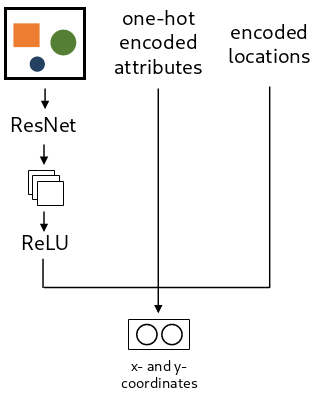
\includegraphics[width=0.35\linewidth]{figures/arch_coordinate_predictor.png}
        \label{fig:coordinate_predictor_architecture}
    }
    \subfigure[Model including GRE description]{
        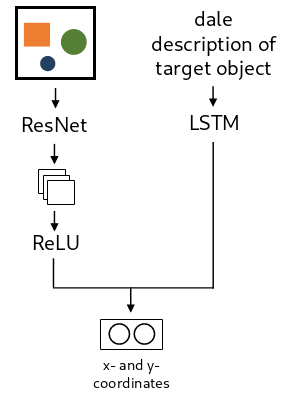
\includegraphics[width=0.315\linewidth]{figures/arch_coordinate_predictor_dale.png}
        \label{fig:coordinate_predictor_dale_architecture}
    }
    \caption{Simplified architecture of the coordinate predictors}
    % SD: How are these encoded?
    % DK: TODO
\end{figure}

In the first method, the target object is encoded as \textbf{one-hot encodings}, as described in section \ref{sec:object-identification}.
In an extension to this method, also the \textbf{center coordinates of all objects} in the image are included.
% SD: Encoded locations?
% DK: TODO
This should help the model to identify all possible options to chose from, when predicting the target object.
All the center coordinates are simply extracted and shuffled.
Since there are varying numbers of objects in the image, this vector of variable length is padded to the maximum number of objects in the dataset.
The padded locations consist of two zeros for both coordinates.
For both methods, the encodings of the target object are concatenated with the encoded image and then passed to the coordinate predictor.
% SD: Why shuffled? If we order them the way they appear in the image, the model will have more information that they are sequentially related.
% DK: TODO
% SD: Convolutions are only applied on visual features, not object attribute features and locations.
% DK: TODO

The third method encodes the attributes of the target object with human language using the \textbf{incremental GRE-algorithm}.
This opposes the idea described before, to share as few natural language information as possible with the model.
Still, this approach can help to understand and analyze if the model was able to extract information about the objects and more specifically their attributes from the image.
% SD: The question you are asking is whether it is possible to predict location from the visual appearance of the object. This is highly complex task as it requires quite two step reasoning, identification of features with that attribute, e.g. blue and then locating that feature in the image.
% DK: TODO
If the model is able to match parts of the image with human words it would show that the model learned this attribute.
If the model in a next step can learn this for the whole dataset, this would mean that it could generalize over these attributes and assign them to certain regions in an image.
This insight would help for succeeding models that make use of these learnings without human language.

% Using the algorithm, one can describe an object using its attributes to discriminate it from other objects as efficiently as possible.
% In other words, the object is described unambiguously using the lowest number of words.
% The algorithm assumes that there is an order of importance for attributes, such as shape, color and size.
% This order defines, which attributes can be left out, while still identifying the object uniquely.
% This research relies on the following order from most important to least important: shape, color, size
% Given for example the scene from \ref{fig:clevr-dale-5} with the target object being the \emph{big purple cylinder}.
% Using all three attributes, this description identifies the object perfectly and uniquely.
% Following the algorithm, we could make the description shorter by removing the least important attribute \emph{size} without loosing unambiguity, describing it as the \emph{purple cylinder}.
% This can be taken even one step further by removing also the \emph{color}.
% Describing it as the \emph{cylinder} still doesn't describe any distractor, since the target object is the only cylinder in the scene.
% % SD: See my point earlier about the reversed algorithm between the two tasks 
% % DK: TODO

For the experiments, each image is captioned with a description of the target object using the described algorithm.
To include it in the model, the captions need to be padded to an equal length.
In this case they are padded to a length of 3, which is the maximum number of attributes that can be used.
For this, as standard practice in captioning tasks, the captions are padded at the end with a specified padding token.

In the model, the referring expression is encoded, using an LSTM.
Here, the learned embeddings of each token are parsed by the LSTM and its final hidden state is then used as a summary of the complete caption.
Tokens are embedded with embedding dimensions $LSTM_e$ and the output of the LSTM has the size if $LSTM_o$.
The vocabulary that is used for the descriptions is based on 14 symbols, including the padding token.
Both the processed image and the final hidden state of the LSTM are flattened and concatenated, which is then passed through the coordinate predictor.
% SD: \citep and \citet Use Name (year) when you are referring to particular person and (Name, year) when you are referring to a paper. Hence, in this case it would be the latter.
% DK: done

The fourth method, to encode the target object utilizes \textbf{masking} of the image.
% SD: Oh, before we talked about 3 methods
% DK: done
The image is masked in the same way as in section \ref{sec:referring_expression_generation}.
While even the one-hot encodings contain human knowledge by explicitly encoding human chosen attributes, masking the image will only point the model towards the target object without giving more information.
It therefore can only rely on its own extracted visual features and the inherent human bias in the image when looking at masked images.
% SD: The information in the masked image is still not enough to identify the precise location, only the region. Hence, it corresponds on attention in the attention models. But those are generating labels and not predicting coordinated. The task is still challenging.
% DK: TODO
Both original and masked image are processed as described in \ref{sec:image-processing} and afterwards passed through the coordinate predictor.

For all setups, the same hyperparameters as in the previous experiments are used: a learning rate of $2\times10^{-4}$, a batch size of 32 samples and 30 epochs, \emph{Adam} \citep{Kingma2015} as optimizer.
8000 randomly selected samples are used for training, the remaining 2000 samples for testing.
The loss is calculated using cross entropy.
Table \ref{tab:variables-reference-resolution} shows the variables that are changed during the experiments for each of the models.

\begin{table}[ht]
    \centering
    \begin{tabular}{lcccc}
        \toprule
                               & $e_i$              & $c$               & $LSTM_e$  & $LSTM_o$               \\
                               & $[100, 500, 1000]$ & $[512,1024,2048]$ & $[15,30]$ & $[500,1000,1500,2000]$ \\\midrule
        reference resolver     & \times             & \times            & -         & -                      \\
        + one-hot              & \times             & \times            & -         & -                      \\
        + one-hot + locations  & \times             & \times            & -         & -                      \\
        + referring expression & \times             & \times            & \times    & \times                 \\
        + masking              & \times             & \times            & -         & -                      \\
        \bottomrule
    \end{tabular}
    \caption{Variables for each model where $e_i$ is the image embedding dimension, $c$ the dimensions of the coordinate predictor, $LSTM_e$ the embedding dimensions for tokens in the LSTM and $LSTM_o$ the output dimension of the LSTM}
    \label{tab:variables-reference-resolution}
\end{table}

The test dataset is again evaluated on the euclidean distance of the predicted coordinates to the ground truth coordinates.
This distance needs to be minimized.
The mean of all calculated distances is calculated across the whole epoch, which results in a mean distance score per epoch.
Since this score only takes the average of all predictions into account it doesn't show how every prediction fared individually.
If for instance the prediction of one object is getting more precise with growing number of epochs, but the precision of another object gets worse, the mean distance will stay the same.
% SD: Yes that’s correct but through several epochs we hope we will refine the distance and standard deviation of the error. It should level out. It is not a problem. What you do with a circle and accuracy is that you make the task easier as your pointer is now not pointing to a point but to a larger area.
% DK: TODO
It doesn't reflect this change.
For that reason, we also introduced an accuracy score.
For that we defined a fixed size circle with a radius of 20 pixels around the center of each object.
If the model's prediction lies in this circle, it will be counted as a correct prediction, if it lies outside, it is a false prediction.
These scores are averaged for the epoch and result in an accuracy score, where 100\% means that all predictions were very close to the center coordinates and 0\% means that no predictions were close to the center coordinates.
% SD: But here the score will face the same problem with steward deviation. Hence the only difference here is that pointing is less precise.
% DK: TODO
This of course doesn't give a perfect representation since the size of the objects varies, but it will still show, how precise each individual prediction is.
A high accuracy may indicate that the model could identify this specific object better.

The reference resolution models are trained on the 'CLEVR single' as well as on both 'Dale' datasets.
The 'CLEVR single' dataset should test the model if it can actually learn locations of an object.
Since the model relies on the extracted features of either VGG or ResNet, locational information about the image could have gone lost.
% SD: Explain. w3 had a paper with John Kelleher on what spatial information is encoded in CNNs
% DK: TODO
Training on this dataset should make sure that the model can converge towards the correct pixels, utilizing these features.
In a next step, the 'Dale' datasets provide the actual problem of discriminating objects from each other and afterwards pointing to the correct one.
Here, the models should make use of the additional given referring expressions about the scene, as one-hot encodings of the attributes, descriptions using the GRE-algorithm or the encoded locations.
'Dale-2' and 'Dale-5' provide two different difficulties for the model, where it needs to discriminate a target object from one or four distractors.
% SD: Point at not just discriminate
% DK: TODO
Latter task is assumed to be significantly harder.

\subsubsection*{Results}

\begin{figure}[ht]
    \centering
    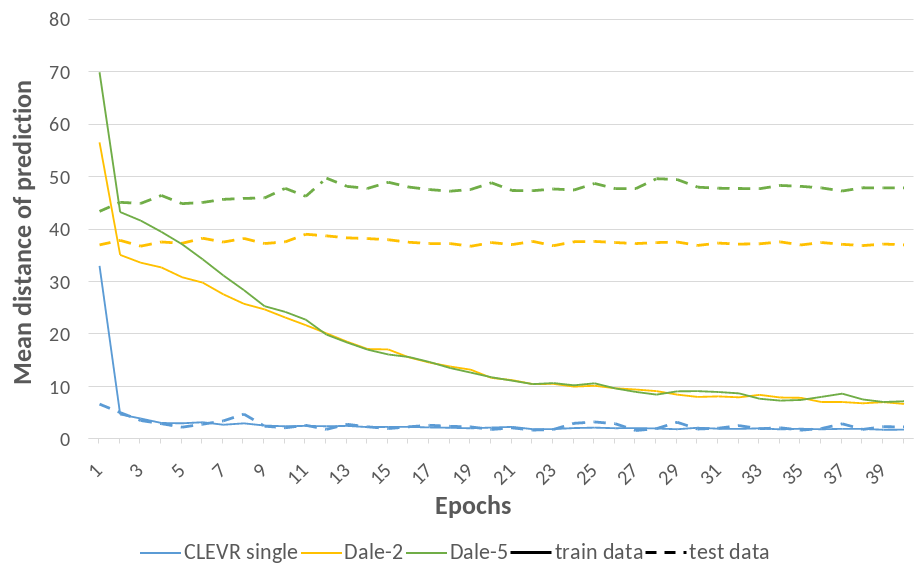
\includegraphics[width=0.8\linewidth]{figures/coordinate-predictor_loss.png}
    \caption{Mean distance between predicted coordinates and ground truth in pixels on different datasets}
    \label{fig:coordinate-predictor_loss}
\end{figure}

Figure \ref{fig:coordinate-predictor_loss} shows the results of the coordinate predictor that doesn't include any information about the target object.
The used feature extractor for these results is \emph{Resnet-3}, but the results don't differ meaningfully from results with other feature extractors.
As can be seen, the success between the different datasets are significant.
The more objects are present in an image, the worse the model performs.
The model converges for the CLEVR single dataset after around 20 epochs to a mean distance of around 2 pixels.
This prediction even though not perfectly on the center point is always on the object.
Opposed to that, using the Dale-2 dataset with two objects, the mean distance lies between 37 and 38 pixels already after the first epoch and doesn't drop with increasing number of epochs.
With five objects in the Dale-5 dataset, the model only predicts a mean distance of around 45 pixels in the beginning, which worsens with a rising number of epochs to 48 pixels.

An interesting observation is the difference of the mean distances between training and testing data.
% SD: How can we have epochs on the testing data? There is no updates so i5 does not make sense.
% DK: TODO
The training distance is constantly approaching zero, while the testing loss is staying constant or even getting higher.
This points to the fact that the model is not generalizing the task by learning abstract patterns that can be applied to unseen data, but is instead memorizing the training data.
That is especially visible for the Dale-5 dataset, where learning the patterns of the training data looses even the ability to interpret some patterns in the testing data.
Applying a higher dropout didn't have an impact on the results.
% SD: The results show that the model is learning something from the training data but this is not the feature that should be learning as the performance on the test data is low. Actually, is it low, it is 10, 35 and 45 pixels. We should not expect any difference between epochs as there is no training. Hence, a flat line is expected.
% DK: TODO

This behavior is indeed not very surprising.
First, results with the 'CLEVR single' dataset show that the model is able to derive geometrical information from abstract feature, extracted by a feature extractor.
Geometrical information therefore doesn't get lost during this abstraction, but the model is able to point to a specific object, as long as only one object is part of the image.
% SD: Because it is in the same location?
% DK: TODO
Secondly, more than one objects present in an image confuses the model, and it is not able to consistently point to one of them.
This can have multiple reasons, for instance that the models lacks the ability to separate objects in the extracted features.
But even in case, the model is able to do that and could determine the location of each object in the scene given the feature, it would not be able to tell, which of these is the actual target object.
The guess is then more or less random.
This especially applies to the Dale-2 dataset, where an identification of the target object just based on one distractor is impossible; both of the present objects are unique.
For the Dale-5 dataset, the model could in theory learn that the target object is always the one object which is unique in respect to its and the distractors' attributes.
This task on the other hand seems very difficult to learn.
In conclusion, the models are able to predict geometrical coordinates, but need more information about the target object to identify it.

When the target object \textbf{attributes are encoded as one-hot vectors} and added to the input, the results don't improve.
One factor that now has a much higher impact is the feature extractor that is used.
Table \ref{tab:feature-extractor-mean-distances} compares the mean distances the models predict for the different feature extractors.
The results are shown for the models trained on the Dale-2 and Dale-5 datasets for training and test data.
First, a big difference can be seen between the datasets.
The models only converge to a minimum mean distance of around 46 pixels to the correct coordinates for the Dale-5 dataset, looking at the test data.
In most cases, it stays above 50 pixels.
% SD: What is the image size? What is the size of a typical object? 50 sounds quite good. Attention is predicting one of 7x7 blocks. Is 50 more or less than 1/7 of an image? 
% DK: TODO
Using the Dale-2 dataset, the behavior is a little different.
All ResNet extractors with four residual blocks and an additional average pooling and optionally a classifier layers reach similar scores as the experiments before without any one-hot encodings.
Interestingly, without the classifier layer, the model doesn't converge at all and the mean distances jump up and down between the epochs.
This effect also applies when using less residual blocks.
Using the VGG, only VGG-cls2 achieve a similar performance, while the others predict coordinates between 43 and 46 pixels away.

\begin{table}[ht]
    \centering
    \begin{tabular}{rcccc}
        \toprule
                            & \multicolumn{2}{c}{\textbf{Dale-2}} & \multicolumn{2}{c}{\textbf{Dale-5}}                                   \\\cmidrule(lr){2-3}\cmidrule(lr){4-5}
                            & train                               & test                                & train          & test           \\\midrule
        \textbf{VGG-0}      & 30,27                               & 46,20                               & \textbf{32,17} & 54,40          \\
        \textbf{VGG-avg}    & \textbf{29,99}                      & 45,08                               & 32,32          & 52,67          \\
        \textbf{VGG-cls1}   & 37,99                               & 43,28                               & 46,57          & 50,75          \\
        \textbf{VGG-cls2}   & 38,87                               & \textbf{39,02}                      & 47,48          & 49,91          \\
        \textbf{VGG-cls3}   & 39,99                               & 44,32                               & 47,26          & \textbf{46,77} \\\midrule
        \textbf{ResNet-3}   & 78,26                               & 65,23                               & 92,07          & 91,12          \\
        \textbf{ResNet-4}   & 44,14                               & 55,24                               & \textbf{36,48} & 58,28          \\
        \textbf{ResNet-avg} & \textbf{33,06}                      & \textbf{39,18}                      & 47,64          & 46,38          \\
        \textbf{ResNet-cls} & 37,57                               & 38,10                               & 44,72          & \textbf{45,92} \\
        \bottomrule
    \end{tabular}
    \caption{Mean test losses for different feature extractors with one-hot attribute encodings after 20 epochs}
    \label{tab:feature-extractor-mean-distances}
    % SD: Explanation of labels
    % DK: TODO
\end{table}

Secondly, the training loss now looks also different.
In almost no cases, the models converge to a lower mean distance than with the test data, meaning a higher precision in their predictions, as they did in the experiment before.
The only exception is ResNet-3 as a feature extractor.
In other words, the models are again not able to generalize, but in specific cases memorize the patterns in the train data.
This hints to the fact that only specific layers of the feature extractors contain information that is generally usable to identify and discriminate objects.
Especially the lower layers with fewer residual blocks in the case of ResNet and no classifier layers for the VGG seem to not encode knowledge that can be utilized for this task.
Higher layers, with more specific encoded information need to be used for this research.
The experiments in the following sections are set up using these higher layers.

Adding \textbf{information about the center coordinates} of all objects should have helped the models to get a list of possible predictions.
In theory, the model could learn to choose between these coordinates by relating them to the extracted features of the image.
This hypothesis doesn't hold.
All results for both datasets Dale-2 and Dale-5 are the exact same as without included information about the locations.
The problem therefore doesn't seem to lie in predicting coordinates in general, but predicting the coordinates of the target object.
% SD: Perhaps arranging the objects sequentially would help the model learn spatial contiguity, see my earlier comment.
% DK: TODO
The model is still not able to understand, which object is the target object.
For that reason, a better representation of the target object is necessary.

In a next step, information about the attributes is included using the \textbf{\emph{GRE-algorithm}} from \citet{Dale1995}.
Again, the mean distance of the predictions as well as the accuracy doesn't improve compared to the previous experiments.
% SD: Table with these results?
% DK: the table would show the same figures as the existing table. Should be still included? (QUESTION)

\begin{figure}[ht]
    \centering
    \subfigure['Dale-2', train split]{
        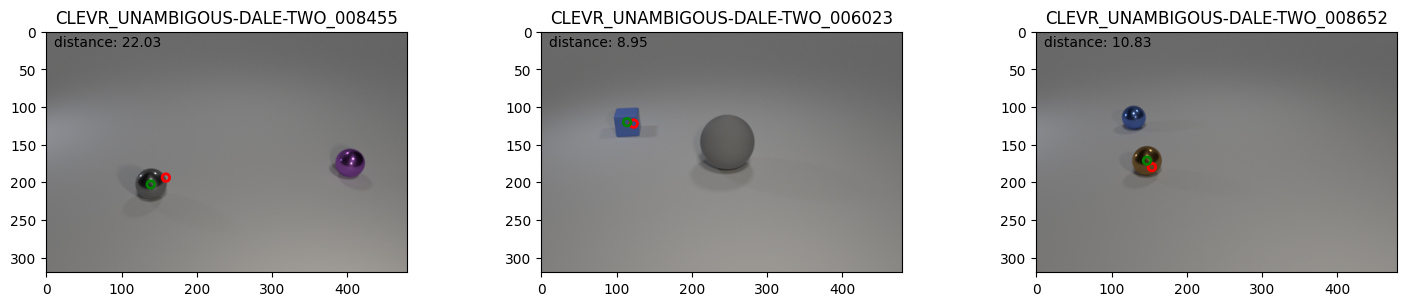
\includegraphics[width=.92\linewidth]{figures/visualization_dale-2_train.png}
        \label{fig:visualizations_dale-2_train}
    }
    \subfigure['Dale-2', test split]{
        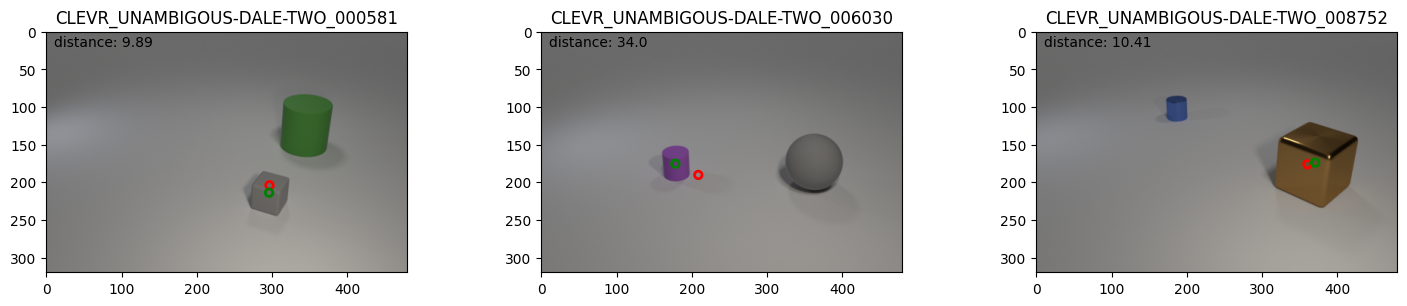
\includegraphics[width=.92\linewidth]{figures/visualization_dale-2_test.png}
        \label{fig:visualizations_dale-2_test}
    }
    \subfigure['Dale-5', train split]{
        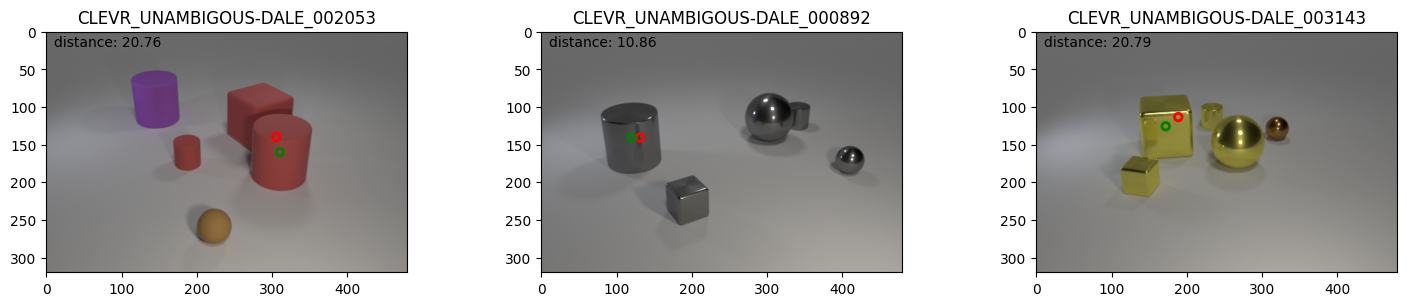
\includegraphics[width=.92\linewidth]{figures/visualization_dale-5_train.png}
        \label{fig:visualizations_dale-5_train}
    }
    \subfigure['Dale-5', test split]{
        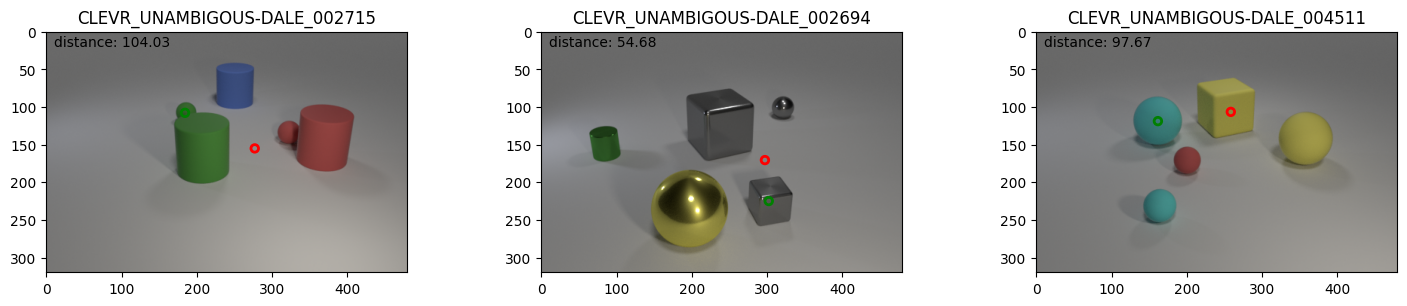
\includegraphics[width=.92\linewidth]{figures/visualization_dale-5_test.png}
        \label{fig:visualizations_dale-5_test}
    }
    \caption{Visualization of the models' predictions in the 'Dale' datasets}
    \label{fig:visualizations_dale}
\end{figure}

An interesting pattern appears when doing a qualitative analysis of the models' predictions.
Here, we visualized the predicted coordinates compared to the ground truth coordinates.
Figure \ref{fig:visualizations_dale-2_train} shows random examples of predictions for images in the train dataset of Dale-2.
The green circle shows the ground truth center coordinates of the target object, while the red circle shows the prediction of the model.
As can be seen, the predictions are very precise.
Figure \ref{fig:visualizations_dale-2_complete_train} combines the predictions and ground truths across all images in the train dataset.
This shows general patterns of the models predictions over the complete dataset.
Here, all predicted coordinates are placed as red circles into the image, while all ground truth coordinates are placed as green circles.
The resulting shape is a rhombus, which reflects that all objects are placed usually central into the scene.
As expected the green and red rhombus align mostly in the same area for the train split of the 'Dale-2' dataset.
% SD: But this image does not show clearly whether the circles for the same object match. You could calculate the average error in distance between the ground truth and predicted coordinates.
% DK: that is done in the quantitative analysis (mean square error above). The visualization should show general learned patterns of the model (as in this case predictions toard the center)

The results look very different for the test split.
As can be seen in Figure \ref{fig:visualizations_dale-2_test}, the three randomly selected predictions don't align with the ground truth coordinates.
For all the images, the predictions don't lie on any object.
In the left image as well as in the central image, the predictions are closer to the target object than towards the distractor, but are still quite imprecise.
% SD: They are closer to the target than distractor and you can see that it is working to a point. But remember this task is very challenging and I wouldn't say the results are so negative.
% DK: right, this is addressed in the conclusions below
These findings align with the mean distance scores, described in the sections before.
However, it seems that the model's predictions are all towards the center of the image.
This can be seen clearer in Figure \ref{fig:visualizations_dale-2_complete_test}.
Again, the green circles form the shape of rhombus.
In contrast, the predictions in red almost all cluster in the center of the image.
They form roughly the shape of a smaller rhombus.
% SD: There is a bias towards the centre but I would not say that the model has not learned anything. I'm surprised that it works so well given the feature representation we have, i.e. no geometric features.
% DK: again, conclusion below
This behavior can be observed for all datasets and architectures of the model.
Figures \ref{fig:visualizations_dale-5_train}, \ref{fig:visualizations_dale-5_test}, \ref{fig:visualizations_dale-5_complete_train} and \ref{fig:visualizations_dale-5_complete_test} show the results for the 'Dale-5' dataset.
Here, the model more likely predicts the center coordinates of a distractor object as seen in the right image, which is also reflected in the lower score of the mean distance.
Also the combined visualization shows the same clustering of predictions in the center of the scene, but the pattern of the smaller rhombus is more visible.
% SD: The centre bias could be the way the error function is used, that is averages all distances and of course this has a tendency to some middle distance. A solution would be to have better geometric features that could take these errors better into account.
% DK: TODO (future work)

\begin{figure}[ht]
    \centering
    \subfigure['Dale-2', train split]{
        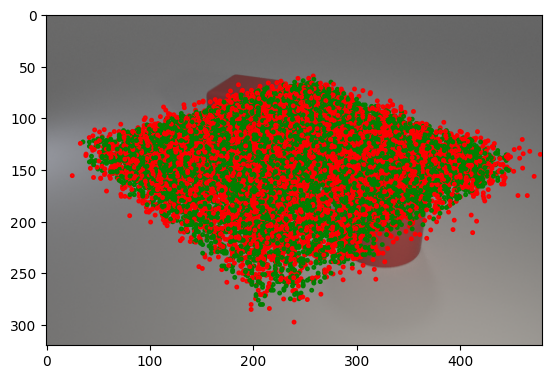
\includegraphics[width=0.42\linewidth]{figures/visualization_dale-2_train_complete.png}
        \label{fig:visualizations_dale-2_complete_train}
    }
    \subfigure['Dale-2', test split]{
        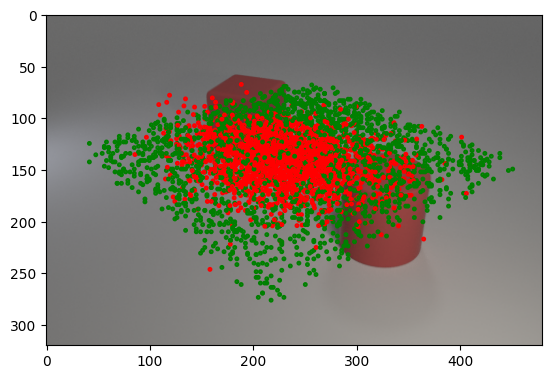
\includegraphics[width=0.42\linewidth]{figures/visualization_dale-2_test_complete.png}
        \label{fig:visualizations_dale-2_complete_test}
    }
    \subfigure['Dale-5', train split]{
        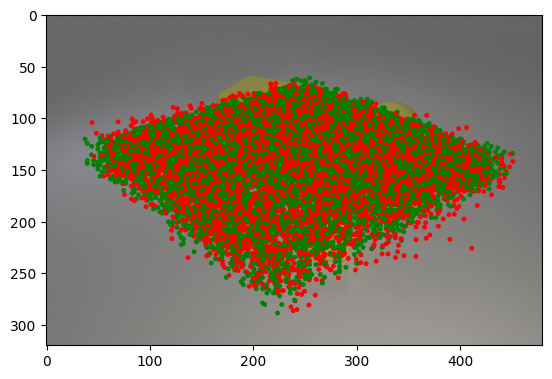
\includegraphics[width=0.42\linewidth]{figures/visualization_dale-5_train_complete.png}
        \label{fig:visualizations_dale-5_complete_train}
    }
    \subfigure['Dale-5', test split]{
        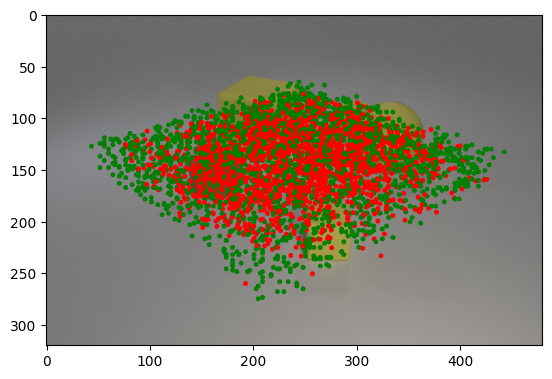
\includegraphics[width=0.42\linewidth]{figures/visualization_dale-5_test_complete.png}
        \label{fig:visualizations_dale-5_complete_test}
    }
    \caption{Visualization of the models' predictions in the Dale datasets}
    % SD: I Haven't checked the earlier captions, but the captions should be informative in the sense that one does not need to look for the text to understand them. Hence, include a brief summary of what each figure contains.
    % DK: TODO
    \label{fig:visualizations_dale_complete}
\end{figure}

These results allow two conclusions.
First, the models are biased to predict coordinates in the center of the image.
% SD: centre - using British English?
% DK: so far I used always American English (hopefully consistently)
The reason for this is likely that the model can produce a relatively low loss, without relying on many extracted features of the objects.
Since all objects are always located in the center of the image and never in its corners, a prediction of any coordinate in the center is on average closer to the target object than any random prediction or predictions of coordinates at the borders of the image.
The model therefore learns only, where any object is likely located and can minimize the mean distance to a certain extent with this strategy.

Second, even though the models are biased towards the center of the image, the predictions are still often leaning towards the location where many objects lie.
This can be seen for the 'Dale-5' dataset, especially in left and central image in Figure \ref{fig:visualizations_dale-5_test}.
Again, by this strategy, the model can minimize the mean distance, since the probability is high that the target object lies in this cluster of objects.
Concluding, the model is able to extract, where objects are located in the image, but can't make use of the referring expressions, to decide which of these objects is the target object.
% SD: There is a centre bias and the model can partially locate the target. The task is hard. The features are not optimal for this task. Future would should focus on using geometric features - we should have tried these and I'm sure we would get better results. Another extension would be making pointing less precise, i.e. focus on a single point, i.e. using a circle of 20 pixels or a 7x7 grid as in the attention mechanism. This would simplify the task.
% DK: TODO (future work)
